\chapter{Slip coefficient and Slip curve of Belt drive}
\section{Nomenclature}
\begin{tabular}[t]{lp{7cm}}
	$ F_{ms} $ & friction force, $ N $\\
	$ F_0 $ & initial tension, $ N $\\
	$ F_t $ & tangential force, $ N $\\ 
	$ Q $ & load, $ kg\cdot F $\\
	$ g $ & gravitational acceleration at sea level, $ m/s^2 $\\
	$ h_i $ & distance between outer sides of the belt before applying load $ Q $, $ mm $\\
	$ h_f $ & distance between outer sides of the belt after applying load $ Q $, $ mm $\\
	$ \Delta h $ & difference between $ h_i $ and $ h_f $, $ mm $
\end{tabular}
\begin{tabular}[t]{lp{7cm}}
	$ n $ & rotational speed, $ rpm $\\
	$ d $ & diameter, $ mm $\\
	$ f $ & coefficient of friction\\
	$ a $ & center distance, $ mm $\\
	$ \alpha $ & wrap angle, $ ^{\circ} $\\
	$ \beta $ & slack angle due to load $ Q $, $ ^{\circ} $\\
	$ \xi $ & slip coefficient\\
	$ \phi $ & drag coefficient\\
	$ \overline{\xi} $ & average slip coefficient $ kW $\\
	$ _1 $ & subscript for driving pulley\\
	$ _2 $ & subscript for driven pulley\\
\end{tabular}\newpage
\section{Purpose}
\begin{enumerate}
	\item Investigate slip in belt drives
	\item Find relative slip coefficient and conduct experiment to find $ \xi $
	\item Find $ F_0 $
	\item Draw slip curve with respect to $ Q $
\end{enumerate}

\section{Safety Procedures}
Students must follow safety rules in the lab.

\section{Conduct Experiment}
\subsection{Find parameters of the experiment kit}
	\begin{itemize}
		\item $ d_1 = 67.8\unit{mm} $, $ d_2 = 165\unit{mm} $, $ a = 315\unit{mm} $
		\item Belt type: flat belt
		\item $ \alpha_1 = 180 - 57\dfrac{d_2-d_1}{a} \approx 162.3^{\circ}$
		\item $ \alpha_2 = 180 + 57\dfrac{d_2-d_1}{a} \approx 197.6^{\circ}$
	\end{itemize}
\subsection{Find $ F_0 $}
	\begin{itemize}
		\item $ h_i = 124\unit{mm}$, $ h_f = 94\unit{mm} $, $ Q = 4.1\unit{kg\cdot F} $
		\item $ \Delta_h=|h_f-f_i|=30\unit{mm} $, $ \beta=\arctan\dfrac{2\Delta_h}{a} \approx 10.78^{\circ}$
		\item $ F_0 = \dfrac{Qg}{2\sin\beta} \approx 107.48\unit{N}$
	\end{itemize}
\subsection{Measurements}
Using the formulas $ \xi=1-\dfrac{d_2n_2}{d_1n_1} $ and $ \phi=\dfrac{F_t}{2F_0} $, we obtain the following table:
\begin{table}[ht]
	\centering
	\begin{tabular}{|c|l|l|l|l|l|l|}\hline
		No. & $ F_0\unit{N}$ & $ n_1\unit{rpm} $ & $ n_2\unit{rpm} $ & $ \xi $ & $ F_t\unit{N} $ & $ \phi $\\\hline
		1 & 107.48 & 283.62 & 114.04 & 0.018 & 3.1 & 0.014\\\hline
		2 & 107.48 & 330.47 & 133.35 & 0.018 & 8.8 & 0.041\\\hline
		3 & 107.48 & 273.83 & 110.27 & 0.02 & 14.4 & 0.067\\\hline
		4 & 107.48 & 307.52 & 123.71 & 0.021 & 20.2 & 0.094\\\hline
		5 & 107.48 & 354.42 & 142.43 & 0.022 & 22.1 & 0.103\\\hline
	\end{tabular}
	\caption{Observed data}
\end{table}
Averaging the values of $ \xi $ yields $ \overline{\xi} \approx 0.0198$
\subsection{Draw the slip curve graph}
From the data above, we can approximate the best fitted line through the data points (assuming linearity since $ \phi $ does not reach critical value)
\begin{figure}[ht]
	\centering
	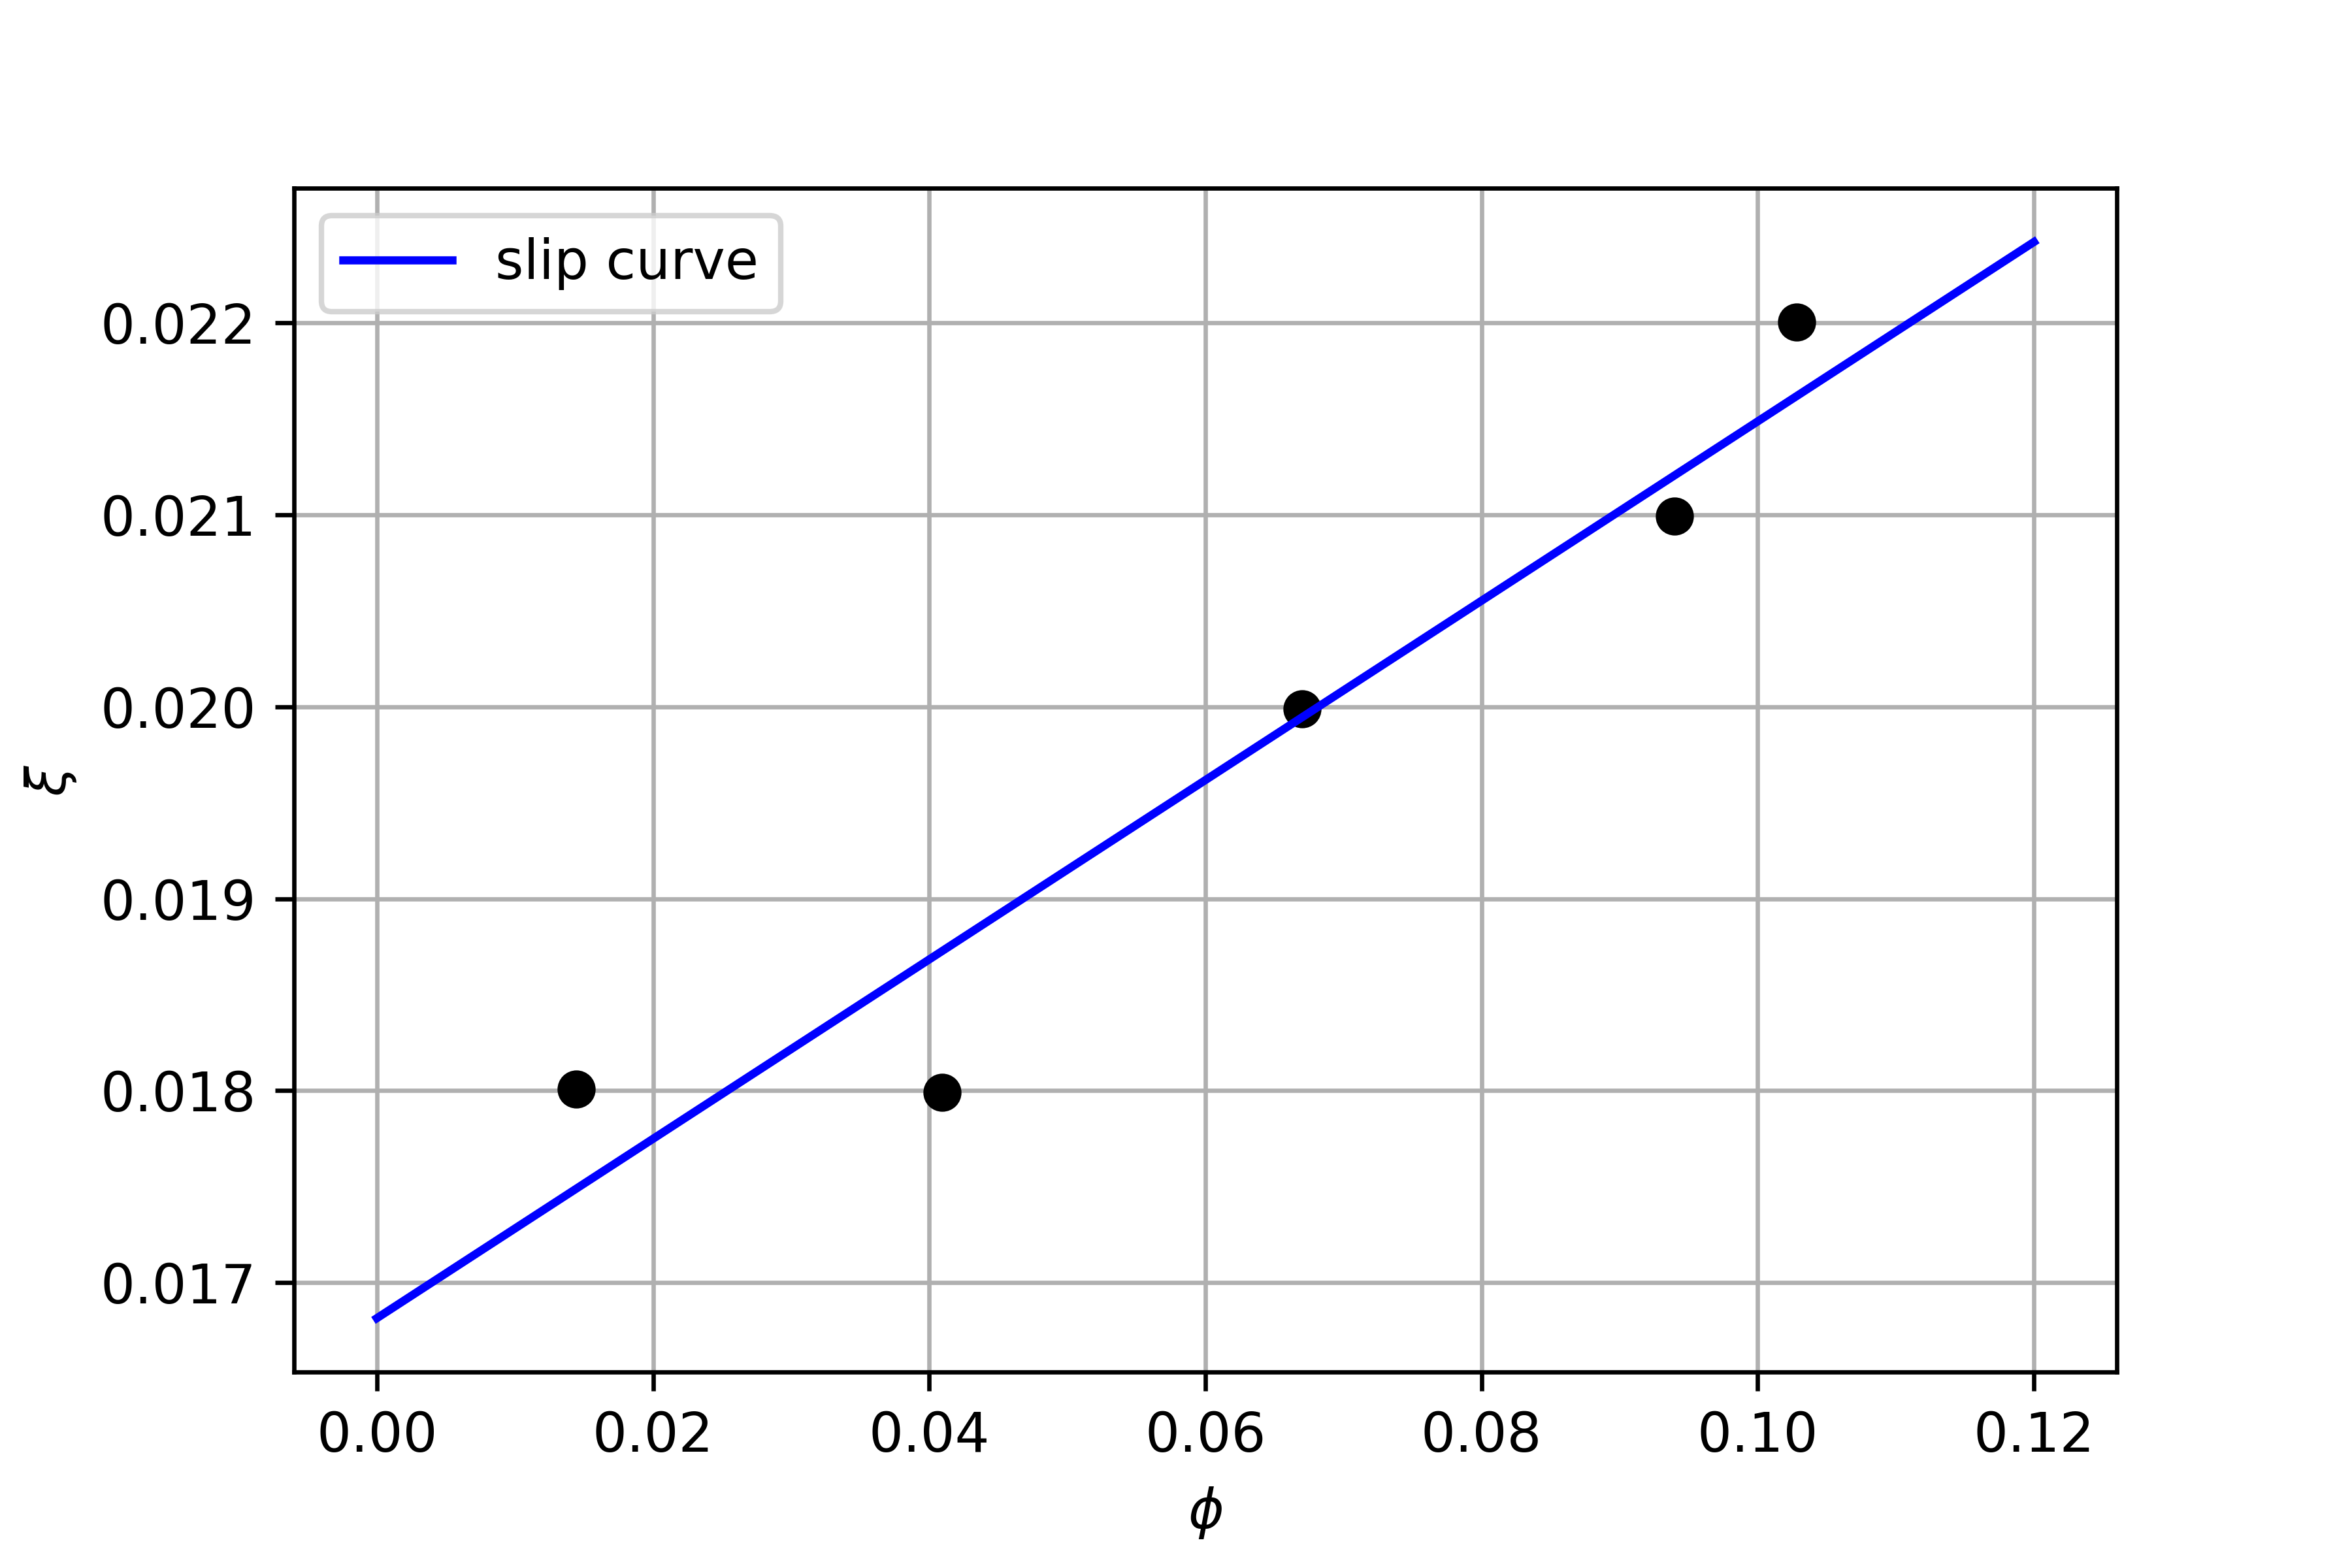
\includegraphics{Exp1.png}
	\caption{Slip curve of belt drive}
\end{figure}

\section{Conclusions}
In summary:
\begin{itemize}
	\item Slip coefficient from experiment is in allowable range ($ 0.01\div0.02 $).
	\item The slip curve is in agreement with theory (error is smaller than $ 5\% $). Since $ \phi $ does not exceed critical value (the motor is frequency-controlled), we can safely assume linearity for the curve.
	\item Possible errors:
	\begin{itemize}
		\item manually measure dimensions in the kit.
		\item rounding.
		\item incorrect reading of rotational speeds.
	\end{itemize}
	\item The slip coefficient and slip curve is considerably accurate due to reliable instrument
\end{itemize}
\section{Review questions}
\begin{enumerate}
	\item There are 
\end{enumerate}